\documentclass[a4paper,10pt]{article}

\usepackage[activeacute]{babel}
\usepackage[utf8]{inputenc}
\usepackage{bookman}
\usepackage{color}
\usepackage{graphicx}
\usepackage{anysize}
\usepackage{multicol}
\usepackage[pdftex=true,colorlinks=true,linkcolor=black,urlcolor=blue]{hyperref}

\marginsize{1.5cm}{1.5cm}{1.5cm}{1.5cm}
\newcommand{\HRule}{\rule{\linewidth}{0.5mm}}

\date{}

\pagenumbering{arabic}
\setcounter{page}{1}

\begin{document}

% ===================================== MEMBRETE ===================================== %
\begin{center}
  \textsc {
    Universidad Simón Bolívar \\[0cm]
    Departamento de Computaci\'on y Tecnolog\'ia de la Informaci\'on \\[0cm]
    CI5438 - Inteligencia Artificial I \\[0cm]
    Trimestre Abril - Julio 2021 \\[0cm]
    Prof. Carlos Infante \\[0cm]
    Amin Arriaga 16-10072, David Segura XX-XXXXX, Wilfredo Graterol XX-XXXXX
  }
  \HRule \\[0.4cm]
  {\Large \textbf{B\'usqueda Informada: A* vs IDA*}} \\[0.4cm]
  \textsc{
    \today
  }
  \HRule
\end{center}

\section{15Puzzle}
  Para el \textit{15Puzzle} usamos como heur\'istica la distancia Manhattan.

  
  \begin{verbatim}
  STATE (EASY):   14 1 9 6 4 8 12 5 7 2 3 B 10 11 13 15
  |           FUNCTION|   TIME (SEC)|  MEMORY (GB)|       NODES/SEC|    SOL-LEN|
  |                 A*|   172.613782|      5.39361|    138210.58622|         45|
  |         A* pruning|     2.627228|      0.04398|     62283.51708|         45|
  |    A* late pruning|     2.593914|      0.04016|     90053.48674|         45|
  |               IDA*|   294.174137|      0.00055|    243362.32182|         45|
  |       IDA* pruning|     1.537629|       0.0129|    410535.96154|         45|
  |  IDA* part pruning|     2.629333|      0.00024|    240086.36411|         45|
  \end{verbatim}        
  
  \begin{verbatim}  
  STATE (MEDIUM): 12 9 B 6 8 3 5 14 2 4 11 7 10 1 15 13                                                                                       
  |           FUNCTION|   TIME (SEC)|  MEMORY (GB)|       NODES/SEC|    SOL-LEN|
  |                 A*|                    TOO MUCH MEMORY                     |
  |         A* pruning|   361.748725|      2.56905|     26938.20137|         50|
  |    A* late pruning|   184.561287|      2.34054|     85301.65917|         50|
  |               IDA*|                     TOO MUCH TIME                      |
  |       IDA* pruning|   243.698492|      0.00148|    413353.29231|         50|
  |  IDA* part pruning|   421.172057|       0.0001|    239603.34577|         50|
  \end{verbatim}

  \begin{verbatim}  
  STATE (HARD):   5 9 13 14 6 3 7 12 10 8 4 B 15 2 11 1                                                                                     
  |           FUNCTION|   TIME (SEC)|  MEMORY (GB)|       NODES/SEC|    SOL-LEN|
  |                 A*|                    TOO MUCH MEMORY                     |  
  |         A* pruning|   633.547779|       4.1973|     25436.99234|         57|
  |    A* late pruning|   305.977159|      3.92621|     77683.54042|         57|
  |               IDA*|                     TOO MUCH TIME                      |
  |       IDA* pruning|   349.547181|      0.00082|    404336.85832|         57|
  |  IDA* part pruning|   591.625852|      0.00195|    238931.14461|         57|
    \end{verbatim}

  \begin{figure*}[h!]
    \centering
    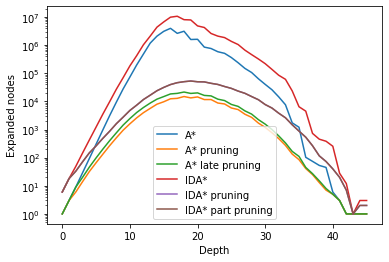
\includegraphics[scale=0.6]{15puzzle_easy.png}
    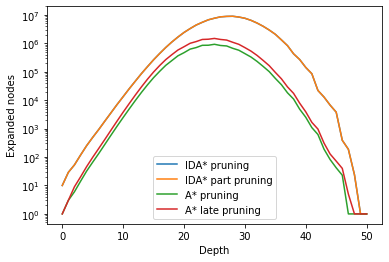
\includegraphics[scale=0.6]{15puzzle_medium.png}
    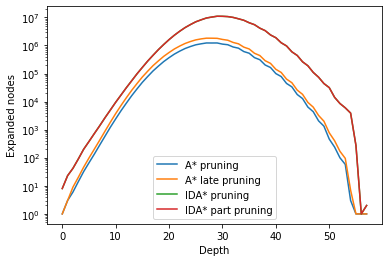
\includegraphics[scale=0.6]{15puzzle_hard.png}
    \\
    \small{\textit{Figure 1: Left, easy. Right, medium. Down, hard}}
  \end{figure*}  

\end{document}